\section{Introduction}

\say{Remember your readers, especially your 2nd marker might have no knowledge of the topic of your project. The introduction is your chance to tell them what your project is about. What is the topic of your project? What are the problems? Why is it important? In the introduction you are trying, at a high-level to give the reader an idea of these issues. Convince them that your project is something interesting that's worth working on.}

% \gls{latex}
% \acrshort{fpt}

\begin{enumerate}
    \item What is the general problem?
          \begin{itemize}
              \item Parameterized Streaming Algorithms for k-VC
                    \begin{enumerate}
                        \item $2^k$-Pass BST using $O(k \cdot \text{log } n)$ bits
                              % \begin{figure}[h]
                              %     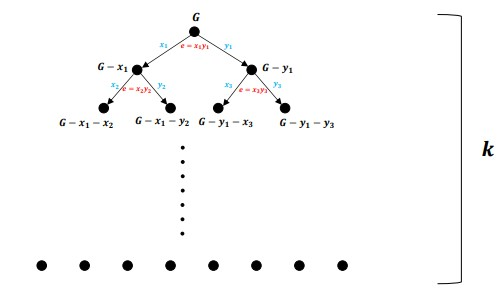
\includegraphics{2^k-pass-bst}
                              %     \centering
                              % \end{figure}
                        \item $1$-Pass BST using $O(k^2 \cdot \text{log } n)$ bits
                        \item Greedily maintain Maximal Matching $O(k^2)$ stored vertices and edges
                              % \begin{figure}[h]
                              %     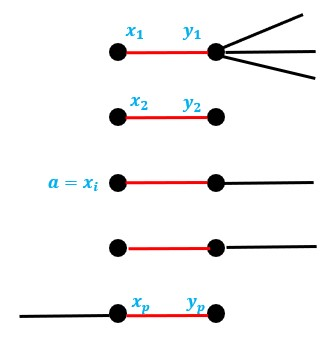
\includegraphics{1-pass}
                              %     \centering
                              % \end{figure}
                        \item $O(k^2)$ Kernel
                    \end{enumerate}
              \item \note{Copied from pdf}Recall that in the classical Vertex Cover problem, the goal is to find a min vertex cover. In the parameterized Vertex Cover problem, given a parameter k, we only want to know if $G$ has a vertex cover of size $\leq k$ or not. The goal is to develop fast algorithms when $k$ is small, even if the input size $n$ is large.
              \item Definition: A parameterized problem with parameter $k$ and input size $n$ is said to be fixed-parameter tractable (FPT) if it can be solved in time $f(k) \cdot n^{O(1)}$, for some function $f$.
          \end{itemize}
    \item Why is it worth working on?
          \begin{itemize}
              \item Graphs have been shown to be excellent models for real world situations
              \item Having a low enough algorithmic complexity to be able to solve some problems on graphs allows us to solve real world problems
          \end{itemize}
    \item Who else as worked on this problem?
          \begin{itemize}
              \item Rajesh Chitnis et al
          \end{itemize}
    \item What did they find?
          \begin{itemize}
              \item That this works in theory
          \end{itemize}
    \item Given this, what is the specific problem you will solve?
          \begin{itemize}
              \item Showing their performance vs real world datasets
          \end{itemize}
\end{enumerate}

\todo[inline]{Talk more about the work Rajesh has done}

My supervisor Rajesh Chitnis had previously been researching the problem of parameterized vertex cover. I found that none of the algorithms he talked about had ever been put into practice, only ever written theoretically.

\subsection{The Problem}

Parameterized Streaming Algorithms for the Graph Theory problem of Vertex Cover. That is the problem. Let me break that down into its individual parts.

Graph Theory: the study of mathematical structures which are used to show pairwise relations between objects.

Vertex Cover: a set of vertices such that each edge of a graph is incident to at least one vertex of the set. The problem of finding a minimum vertex cover (the smallest possible) is a classical optimization problem and is a typical example of an NP-hard problem. The decision version (where we only want a yes/no answer), known as the Vertex Cover Problem, is one of Karp's 21 NP-complete problems. This makes is a very classical problem. Formally, given a graph \(G = (V, E)\) and a vertex cover \(V'\):

\[V' \subset V \text{ such that } \forall (u, v) \in E \Rightarrow u \in V' \vee v \in V' \]

Parameterized complexity: A branch of computational complexity theory that focusses on classifying computational problems according to their inherent difficulty with respect to multiple parameters of the input or output. The complexity of the problem is then measured as a function of those parameters. The vertex cover problem is fixed-parameter tractable, meaning that, while it may be NP-complete in terms of the input size only, it is polynomial in the output of a vertex cover size \emph{k}.

Streaming Algorithms: We now live in a world where data is the most valuable resource. Given such, it's no surprise that we're drowning in it. Datasets have become larger than what we can store on hard drives. The solution is to not store the dataset. Simply stream it as one item at a time. Streaming algorithms have been developed to handle this, being able to gather information while having access to a limited amount of memory.

\subsection{Why is this important?}

Vertex cover is a classical problem which has found many use cases. Here's a typical example. Imagine a heavily connected road network in a city. The city council wants to figure out the most cost effective placement of cameras so that they are able to see every road (assume the cameras can see 360$^\circ$). The way of calculating this mathematically would be as a vertex cover of a graph where each intersection was a node and each road between them is an edge. For cities nowadays, this graph can be too big to compute using traditional methods. So we need updated methods to handle this.

\subsection{Previous Contributions}

\begin{itemize}
    \item \cite{chitnis_parameterized_2014}
    \item \cite{chitnis_kernelization_2015}
\end{itemize}

\subsection{What I Plan To Contribute}

\subsubsection{Implementation of algorithms}
\subsubsection{Typical use cases}
\subsubsection{Implementation of use cases}
\subsubsection{Proof-of-concept production environment (Kafka)}
\subsubsection{Analysis and comparison of algorithmic complexity}
\subsubsection{Platform on which to build further research into graph streaming algorithms}
